\documentclass[../main.tex]{subfiles}
\begin{document}

\section{Topological Artist Model}
\label{sec:tam}

As discussed in the introduction, visualization is generally defined as structure preserving maps from data to graphic representation. In order to formalize this statement, we describe the connectivity of the records using topology and define the structure on the components in terms of the monoid actions on the component types. By formalizing structure in this way, we can evaluate the extent to which a visualization preserves the structure of the data it is representing and build structure preserving visualization tools. 
We introduce the notion of an artist $\mathscr{\vartist}$ as an equivariant map from data to graphic
\begin{equation}
    \label{eq:artist}
    \mathscr{\vartist}: \mathscr{\dtotal} \rightarrow \mathscr{\gtotal}
\end{equation}
that carries a homomorphism of monoid actions $\varphi: \monoid \rightarrow \monoid^{\prime}$ \cite{cegarraCohomologyMonoidsOperators2019}, which are discussed in detail in section~\ref{sec:data_monoid}. Given \monoid\ on data $\mathscr{\dtotal}$ and $\monoid^{\prime}$ on graphic $\mathscr{\gtotal}$, we propose that artists $\mathscr{\vartist}$ are symmetric 
\begin{equation}
\mathscr{\vartist}(m\cdot \delement) = \varphi(m)\cdot\mathscr{\vartist}(\delement) 
\end{equation}
such that applying a monoid action $m \in \monoid$ to the input $\delement \in \mathscr{\dtotal}$ to $\mathscr{\vartist}$ is equivalent to applying a monoid action $\varphi(\monoid) \in \monoid^{\prime}$ to the output of the artist $\vartist(\delement) \in \mathscr{\gtotal}$.

We model the data $\mathscr{\dtotal}$, graphic $\mathscr{\gtotal}$, and intermediate visual encoding $\mathscr{\vtotal}$ stages of visualization as topological structures that encapsulate types of variables and continuity; by doing so we can develop implementations that keep track of both in ways that let us distribute computation while still allowing assembly and dynamic update of the graphic. To explain which structure the artist is preserving, we first describe how we model data (\ref{sec:data}), graphics (\ref{sec:graphic}), and intermediate visual characteristics (\ref{sec:artist}) as fiber bundles. We then discuss the equivariant maps between data and visual characteristics (\ref{sec:artist_nu}) and visual characteristics and graphics (\ref{sec:artist_q}) that make up the artist.

\subsection{Data Space \dtotal}
\label{sec:data}
Building on Butler's proposal of using fiber bundles as a common data representation format for visualization data\cite{butlerVectorBundleClassesForm1992, butlerVisualizationModelBased1989}, a fiber bundle is a tuple $(\dtotal,\,\dbase,\,\pi ,\,\dfiber)$ defined by the projection map $\pi$
\begin{equation}
    \label{eq:fiber_bundle}
    \begin{tikzcd}
        \dfiber \arrow[r, hook] & \dtotal \arrow[r, "\pi"] & \dbase
    \end{tikzcd}
\end{equation}
that binds the components of the data in \dfiber\ to the continuity represented in \dbase. The fiber bundle models the properties of data component types \dfiber\ (\ref{sec:data_fiber}), the continuity of records \dbase\ (\ref{sec:data_base}), the collections of records \dsection\ (\ref{sec:data_section}), and the space \dtotal\ of all possible datasets with these components and continuity. 

By definition fiber bundles are locally trivial\cite{spanier1989algebraic,LocallyTrivialFibre}, meaning that over a localized neighborhood we can dispense with extra structure on \dtotal\ and focus on the components and continuity. We use fiber bundles as the data model because they are inclusive enough to express all the types of data described in section~\ref{sec:intro_data}. 

\subsubsection{Variables: Fiber Space \dfiber}
\label{sec:data_fiber}
To formalize the structure of the data components, we use notation introduced by Spivak \cite{spivakSIMPLICIALDATABASES} that binds the components of the fiber to variable names and types. Spivak constructs a set \ftotal\ that is the disjoint union of all possible objects of types $\{\ftype_0, \ldots, \ftype_m\} \in \ftypes$, where \ftypes\ are the data types of the variables in the dataset. He then defines the single variable set \fttype\ 
\begin{equation}
    \label{eq:data_types}
    \begin{tikzcd}
        \fttype \arrow[r] \arrow[d, "\pi_{\fsection}"'] & \ftotal \arrow[d, "\pi"] \\
        \fnames \arrow[r, "\fsection"']                          & \ftypes       
    \end{tikzcd}
\end{equation}
which is \ftotal\ restricted to objects of type \ftype\ bound to variable name \fname. The \fttype\ lookup is by name to specify that every component is distinct, since multiple components can have the same type \ftype. Given \fsection, the fiber for a one variable dataset is
\begin{equation}
    \dfiber = \ftotal_{\fsection(\fname)} = \ftotal_{\ftype} 
\end{equation}
where \fsection\ is the schema binding variable name \fname\ to its datatype \ftype. A dataset with multiple variables has a fiber that is the cartesian cross product of $\ftotal_{\fsection}$ applied to all the columns:
\begin{equation}
F = \ftotal_{\fsection(\fname_{1})}\times \ldots \ftotal_{\fsection(\fname_{i})} \ldots\times \ftotal_{\fsection(\fname_{n})}
\end{equation}
which is equivalent to 
\begin{equation}
    \dfiber= \dfiber_{0} \times \ldots \times \dfiber_{i}\times\ldots\times \dfiber_{n}
\end{equation}
which allows us to decouple \dfiber\ into components $\dfiber_i$.

\begin{figure}[H]
    \begin{subfigure}{.5\textwidth}
        \includegraphics[width=\textwidth]{figures/math/temp_1k.png}
        \caption{}
        \label{fig:fiber_example_plane}
    \end{subfigure}
    \begin{subfigure}{.5\textwidth}
        \includegraphics[width=\textwidth]{figures/math/temp_3f.png}
        \caption{}
        \label{fig:fiber_example_cube}
    \end{subfigure}
    \caption{These two datasets have the same base space \dbase\ of discrete points, but figure~\ref{fig:fiber_example_plane} has fiber  $\dfiber=\reals\times\reals$ which is (time, temperature) while figure~\ref{fig:fiber_example_cube} has fiber $\reals\times\realsp\times\reals$ which is (time, wind=(speed, direction))}
    \label{fig:data_fiber_example}
\end{figure}

For example, the data in figure~\ref{fig:fiber_example_plane} is a pair of times and \textdegree K temperature measurements taken at those times. Time is a positive number of type \texttt{datetime} which can be resolved to floats $\ftotal_{\texttt{datetime}}= \reals$. Temperature values are real positive numbers $\ftotal_{\texttt{float}} = \realsp$. The fiber is 
\begin{equation}
    \ftotal =  \reals \times \realsp 
\end{equation} 
where the first component $F_0$ is the set of values specified by $(\fname=time,\, \ftype=\texttt{datetime},\, \fttype=\reals)$ and $F_1$ is specified by $(\fname=temperature,\, \ftype=\texttt{float},\, \fttype=\realsp)$ and is the set of values $\fttype=\realsp$. In figure~\ref{fig:fiber_example_cube}, temperature is replaced with wind. This wind variable is of type \texttt{wind} and has two components speed and direction $\{(s,d) \in \reals^{2} \mid  0\leq s,\, 0 \leq d \leq 360\}$ . Therefore, the fiber is 
\begin{equation}
    \dfiber = \realsp \times \reals^{2}
\end{equation} 
such that $F_1$ is specified by $(\fname = wind,\, \ftype = \texttt{wind},\, \fttype=\reals^{2})$.  As illustrated in figure~\ref{fig:data_fiber_example}, Spivak's framework provides a consistent way to describe potentially complex components of the input data. 

\subsubsection{Measurement Scales: Monoid Actions}
\label{sec:data_monoid}
Implementing expressive visual encodings requires formally describing the structure on the components of the fiber, which we define by the action of a monoid on the component. While structure on a set of values is often described algebraically as operations or through the actions of a group, for example Steven's scales \cite{stevensTheoryScalesMeasurement1946}, we generalize to monoids to support more component types. Monoids are also commonly found in functional programming because they specify compositions of transformations \cite{yorgeyMonoidsThemeVariations, stievenMonadJustMonoid2020}. 

A monoid \cite{Monoid2021} $\monoid$ is a set with an associative binary operator $\ast:\monoid \times \monoid\rightarrow \monoid$. A monoid has an identity element $e\in \monoid$ such that $e\ast a= a \ast e = a$ for all $a \in \monoid$. As defined on a component of \dfiber, a left monoid action \cite{SemigroupAction2021,ActionNLab} of $\monoid_i$ is a set $\dfiber_i$ with an action $\bullet: \monoid\times \dfiber_i \rightarrow \dfiber_i$ with the properties:
\begin{align*}
    \textbf{associativity}\;& \text{for all } f,g \in \monoid_i \text{ and } x\in \dfiber_i,\, f\bullet(g\bullet x) = (f\ast g) \bullet x\\
    \textbf{identity}\;& \text{for all } x\in \dfiber_i, e\in \monoid_i,\,  e\bullet x = x 
\end{align*}
As with the fiber \dfiber\, the total monoid space \monoid\ is the cartesian product
\begin{equation}
\monoid= \monoid_{0} \times \ldots \times \monoid_{i}\times \ldots \times\ldots \monoid_{n}
\end{equation}
of each monoid $\monoid_{i}$ on $\dfiber_{i}$.  The monoid is also added to the specification of the fiber $(\fname_i,\, \ftype_i,\, \fttype\, \monoid_i)$

Steven's described the measurement scales\cite{stevensTheoryScalesMeasurement1946,leaFormalizationMeasurementScale} in terms of the monoid actions on the measurements: nominal data is permutable, ordinal data is monotonic, interval data is translatable, and ratio data is scalable \cite{weissteinSimilarityTransformation}. For example, given an arbitrary interval scale fiber component $(\fname=temperature,\, \ftype=\texttt{float},\,\fttype=\reals)$ with arbitrarily chosen monoid translation actions actions 
\begin{itemize}
    \item monoid operator addition $\ast = +$
    \item monoid operations: $f: x\mapsto x + 1 $, $g: x\mapsto x + 2  $
    \item monoid action operator composition $\bullet = \circ$
\end{itemize}
By structure preservation, we mean that monoid actions are composable. For the translation actions described above on the temperature fiber, this means that they satisfy the condition
\begin{equation}
    \begin{tikzcd}
        \reals \arrow[rd, "(x+ 1\degree)\circ(x+2\degree)"] \arrow[d, "x+ 1\degree"'] &            \\
        \reals \arrow[r, "x+ 2\degree"']                                   & \reals
    \end{tikzcd}
\end{equation}
where $1\degree$ and $2\degree$ are valid distances between two temperatures $x$. What this diagram means is that either the fiber could be shifted by 1 (vertical line) then by 2 (horizontal), or the two shifts could be combined such that in this case the fiber is shifted by 3 (diagonal) and these two paths yield the same temperature. 

While many component types will be one of the measurement scale types, we generalize to monoids specifically for the case of partially ordered set. Given a set $W=\{mist, \, drizzle, \, rain \}$, then the map $f: W\rightarrow W$ defined by 
\begin{enumerate}
    \item $f(rain) = drizzle$,
    \item  $f(drizzle) = mist$ 
    \item $f(mist) = mist$
\end{enumerate}
is order preserving such that $mist \leq drizzle \leq rain$ but has no inverse since $drizzle$ and $mist$ go to the same value $mist$. Therefore order preserving maps do not form a group, and instead we generalize to monoids to support partial order component types. Defining the monoid actions on the components serves as the basis for identifying the invariance\cite{kindlmann2014algebraic} that must be preserved in the visual representation of the component. We propose equivariance of monoid actions individually on the fiber to visual component maps and on the graphic as a whole.

\subsubsection{Continuity: Base Space $K$} 
\label{sec:data_base}
The base space \dbase\ is way to express how the records in \dtotal\ are connected to each other, for example if they are discrete points or if they lie in a 2D continous surface. Connectivity type is assumed in the choice of visualization, for example a line plot implies 1D continuous data, but an explicit representation allows for verifying that the topology of the graphic representation is equivalent to the topology of the data.  

\begin{figure}[H]
    \includegraphics[width=1\textwidth]{figures/math/k_different_types.png}
    \caption{The topological base space \dbase\ encodes the connectivity of the data space, for example if the data is independent points or on a plane or a sphere}
    \label{fig:base_space_types}
\end{figure}
As illustrated in figure~\ref{fig:base_space_types}, \dbase\ is akin to an indexing space into \dtotal\ that describes the structure of \dtotal.  \dbase\ can have any number of dimensions and can be continuous or discrete. 

\begin{figure}[H]
    \includegraphics[width=\linewidth]{figures/math/k_qspace.png}
    \caption{The base space \dtotal\ is divided into fiber segments \dfiber. The base space \dbase\ acts as an index into the records in the fibers.}
    \label{fig:base_space_div}
\end{figure}

Formally \dbase\ is the quotient space \cite{QuotientSpaceTopology2020} of \dtotal\, meaning it is the finest space\cite{aurouxMath131Introduction} such that every $\dbasepoint \in \dbase$ has a corresponding fiber $\dfiber_k$\cite{QuotientSpaceTopology2020}. In figure~\ref{fig:base_space_div}, \dtotal\ is a rectangle divided by vertical fibers \dfiber, so the minimal \dbase\ for which there is always a mapping $\pi: \dtotal\rightarrow \dbase$ is the closed interval $\left[0,1\right]$. 
As with fibers and monoids, we can decompose the total space into components $\pi:\dtotal_i\rightarrow \dbase$ where
\begin{equation}
    \pi:\dtotal_1\oplus\ldots\oplus \dtotal_i \oplus\ldots \oplus \dtotal_n \rightarrow \dbase
\end{equation}
which is a decomposition of \dfiber. The \dbase\ remains the same because the connectivity of records does not change just because there are fewer elements in each record.
\begin{figure}[ht!]
    \begin{subfigure}{.5\textwidth}
        \includegraphics[width=\textwidth]{figures/math/temp_1k.png}
        \caption{}
        \label{fig:base_example_discrete}
    \end{subfigure}
    \begin{subfigure}{.5\textwidth}
        \includegraphics[width=\textwidth]{figures/math/temp_2f.png}
        \caption{}
        \label{fig:base_example_continuous}
    \end{subfigure}
    \caption{These two datasets have the same (time, temperature) fiber. In figure~\ref{fig:base_example_discrete} the total space \dtotal\ is discrete over points $\dbasepoint \in \dbase$, meaning the records in the fiber are also discrete. In figure~\ref{fig:base_example_continuous} \dtotal\ lies over the continuous interval \dbase, meaning the records in the fiber are sampled from a continuous space.} 
    \label{fig:base_example}
\end{figure}

The datasets in figure~\ref{fig:base_example} have the same fiber of (temperature, time). In figure~\ref{fig:base_example_discrete} the fibers lie over discrete \dbase\ such that the records in the datasets in the fiber bundles are discrete. The same fiber in figure~\ref{fig:base_example_continuous} lies over a continuous interval \dbase\ such that the records are samples from a continuous function defined on \dbase. By encoding this continuity in the model as \dbase\, the data model now explicitly carries information about its structure such that the implicit assumptions of the visualization algorithms are now explicit. The explicit topology is a concise way of distinguishing visualizations that appear identical, for example heatmaps and images.  
 
\subsubsection{Data: Sections \dsection}
\label{sec:data_section}
The section $\dsection: \dbase\rightarrow \dtotal$ is what ties together the base space \dbase\ with the fiber \dfiber. A section is a function that takes as input location $\dbasepoint \in \dbase$ and returns a record $\delement \in \dtotal$. For example, in the special case of a table \cite{spivakSIMPLICIALDATABASES}, \dbase\ is a set of row ids, \dfiber\ is the columns, and the section \dsection\ returns the record \delement\ at a given key in \dbase. For any fiber bundle, there exists a map
\begin{equation}
    \begin{tikzcd}
        \dfiber \arrow[r, hook] & \dtotal \arrow[d, "\pi"'] \\
                          & \dbase \arrow[u, "\dsection"', bend right]
    \end{tikzcd}
\end{equation}
 such that $\pi(\dsection(\dbasepoint)) = \dbasepoint$. The set of all global sections is denoted as $\Gamma(\dtotal)$. Assuming a trivial fiber bundle $\dtotal = \dbase \times \dfiber$, the section is 
\begin{equation}
    \label{eq:section_return}
    \dsection(\dbasepoint) = (\dbasepoint, (g_{\dfiber_{0}}(\dbasepoint), \ldots, g_{\dfiber_{n}}(\dbasepoint)))
\end{equation}
where $g: \dbase \rightarrow \dfiber$ is the index function into the fiber. This formulation of the section also holds on locally trivial sections of a non-trivial fiber bundle. Because we can decompose the bundle and the fiber, we can decompose \dsection\ as 
\begin{equation}
\label{eq:data_section_decompose}
\dsection= (\dsection_0,\ldots, \dsection_i, \dots, \dsection_n) 
\end{equation}
where each section $\dsection_i$ is a variable or set of variables. This allows for accessing the data component wise rather than just as sections on \dbase.

\begin{figure}[H]
    \includegraphics[width=1\linewidth]{figures/math/fiberbundle.png}
    \caption{ Fiber (time, temperature) with an interval \dbase\ basespace. The sections $\dsection_i$ and $\dsection_j$ are constrained such that the time variable must be monotonic, which means each section is a timeseries of temperature values. They are included in the global set of sections  $\dsection_1, \dsection_2 \in \Gamma(\dtotal)$}
    \label{fig:data_sections}
\end{figure}

In the example in figure~\ref{fig:data_sections}, the fiber is $(time, \, temperature)$ as described in figure~\ref{fig:data_fiber_example} and the base space is the interval \dbase. The section $\dsection^{(1)}$ resolves to a series of monotonically increasing in time records of (time, temperature) values. Section $\dsection^{(2)}$ returns a different timeseries of (time, temperature) values. Both sections are included in the global set of sections $\dsection^{(1)}, \dsection^{(2)} \in \Gamma(\dtotal)$.


This model provides a common interface to widely used data containers without sacrificing the semantic structure embedded in each container. For example, the section can be any instance of a univariate numpy array\cite{harris2020array} that stores an image. This could be a section of a fiber bundle where \dbase\ is a 2D continuous plane and the \dfiber\ is $(\reals^{3}, \reals, \reals)$ where $\reals^3$ is color, and the other two components are the x and y positions of the sampled data in the image. Instead of an image, the numpy array could also store a 2D discrete table. The fiber would not change, but the \dbase\ would now be 0D discrete points. These different choices in topology indicate, for example, what sorts of interpolation would be appropriate when visualizing the data. 

There are also many types of labeled containers that can richly be described in this framework because of the fiber. For example, a pandas series which stores a labeled list, or a dataframe\cite{jeff_reback_2020_3715232} which stores a relational table. A series could store the values of $\dsection^{(1)}$ and a second series could be  $\dsection^{(2)}$. We could also fatten the fiber to hold two temperature series, such that a section would be an instance of a dataframe with a time column and two temperature columns. While the series and dataframe explicitly have a time index column, they are components in our model and the index is always assumed to be random keys.

Where this model particularly shines are N dimensional labeled data structures. For example, an xarray\cite{hoyer2017xarray} data that stores temperature field could have a \dbase\ that is a continuous volume and the components would be the temperature and the time, latitude, and longitude the measurements were sampled at. A section can also be an instance of a distributed data container, such as a dask array \cite{rocklinDaskParallelComputation2015}. As with the other containers, \dbase\ and \dfiber\ are defined in terms of the index and dtypes of the components of the array. Because our framework is defined in terms of the fiber, continuity, and sections, rather than the exact values of the data, our model does not need to know what the exact values are until the renderer needs to fill in the image.  


\subsection{Graphic: \gtotal}
\label{sec:graphic}  
We introduce a graphic bundle to hold the essential information necessary to render a graphical design constructed by the artist. As with the data, we can represent the target graphic as a section \gsection\ of a bundle  $(\gtotal, \gbase, \pi, \gfiber)$. The graphic bundle \gtotal\ consists of a base \gbase (~\ref{sec:graphic_fiber}) that is a thickened form of \dbase\, 
a fiber \gfiber (~\ref{sec:graphic_base}) that is an idealized display space, and sections \gsection (~\ref{sec:graphic_section}) that encode a graphic where the visual characteristics are fully specified.

\subsubsection{Idealized Display \gfiber}
\label{sec:graphic_fiber}
To fully specify the visual characteristics of the image, we construct a fiber \gfiber\ that is an infinite resolution version of the target space. Typically \gtotal\ is trivial and therefore sections can be thought of as mappings into \gfiber. In this work, we assume a 2D opaque image $\gfiber=\reals^5$ with elements 
\begin{equation}
(x,\, y,\, r,\, g,\, b) \in \gfiber
\end{equation}
such that a rendered graphic only consists of 2D position and color. To support overplotting and transparency, the fiber could be $\gfiber=\reals^{7}$ such that $(x, y, z, r, g, b, a) \in \gfiber$ specifies the target display. By abstracting the target display space as \gfiber, the model can support different targets, such as a 2D screen or 3D printer. 

\subsubsection{Continuity of the Graphic \gbase} 
\label{sec:graphic_base}
Just as the \dbase\ encodes the connectivity of the records in the data, we propose an equivalent \gbase\ that encodes the connectivity of the rendered elements of the graphic. For some visualizations, \dbase may be lower dimension than \gbase. For example, in a typical 2D display (ignoring depth), a point that is 0D in \dbase cannot be represented on screen unless it is thickened to 2D to encode the connectivity of the pixels that visually represent the point. This thickening is often not necessary when the dimensionality of \dbase\ matches the dimensionality of the target space, for example if \dbase is 2D and the display is a 2D screen. We introduce \gbase\ to thicken \dbase\ in a way which preserves the structure of \dbase. 

Formally, we require that \dbase\ be a deformation retract\cite{RetractionTopology2020} of \gbase\ so that \dbase\ and \gbase\ have the same homotopy. The surjective map $\vindex: \gbase \rightarrow \dbase$ 
\begin{equation}
    \begin{tikzcd}
        \dtotal \arrow[d, "\pi"'] & \gtotal \arrow[d, "\pi"'] \\
        \dbase                   & \gbase \arrow[l, "\vindex"']
    \end{tikzcd}
\end{equation}
goes from region $\gbasepoint \in \gbase_{\dbasepoint}$ to its associated point $\gbasepoint$. This means that if $\vindex(\gbasepoint) = \dbasepoint$, the record at \dbasepoint\ is copied over the region \gbasepoint\ such that $\dsection(\dbasepoint)=\vindex^*\dsection(\gbasepoint)$ where $\vindex^*\dsection(\gbasepoint)$  is \dsection\ pulled back over \gbase. 

\begin{figure}
    \includegraphics[width=1\textwidth]{figures/math/retraction_maps.png}
    \caption{The scatter and line graphic base spaces have one more dimension of continuity than \dbase\ so that \gbase\ can encode physical aspects of the glyph, such as shape (a circle) or thickness. The image has the same dimension in \gbase\ as in \dbase.}
    \label{fig:graphic_retraction_map}
\end{figure}

When \dbase\ is discrete points and the graphic is a scatter plot, each point $\dbasepoint \in \dbase$ corresponds to a 2D disk $\gbase_{\dbasepoint}$ as shown in figure~\ref{fig:graphic_retraction_map}. In the case of 1D continuous data and a line plot, the region \gy\ over a point $\gx_i$ specifies the thickness of the line in \gbase\ for the corresponding \dsection\ on \dbasepoint. The image has the same dimensions in data space and graphic space such that no extra dimensions are needed in \gbase. 

The mapping function \vindex\ provides a way to identify the part of the visual transformation that is specific to the the connectivity of the data rather than the values; for example it is common to flip a matrix when displaying an image. The \vindex\ mapping is also used by interactive visualization components to look up the data associated with a region on screen.  One example is to fill in details in a hover tooltip, another is to convert region selection (such as zooming) on \gbase\ to a query on the data to access the corresponding record components on \dbase.

\subsubsection{Renderering \gsection}
\label{sec:graphic_section}
\begin{figure}
    \includegraphics[width=\textwidth]{figures/math/render.png}
    \caption{To render a graphic, a pixel $p$ is selected in the display space, which is defined in the same coordinates as the x and y components in \gfiber.  The inverse mapping ${\gsection_{xy}}^(p)$ returns a region $\gbase_{p} \subset \gbase$. $\gsection(\gbase_{p})$ returns the list of elements $(x,\,y,\,r,\,g,\,b) \in \gfiber$ that lie over $\gbase_{p}$. The integral over the $(r,\,g,\,b)$ elements is the color of the pixel.}
    \label{fig:graphic_rho_lookup}
\end{figure}

This section describes how we go from a graphic in an idealized prerender space to a rendered image, where the graphic is the section $\gsection: \gbase \rightarrow \gtotal$. It is sufficient to sketch out how an arbitrary pixel would be rendered, where a pixel $p$ in a real display corresponds to a region $\gbase_p$ in the idealized display. To determine the color of the pixel, we aggregate the color values over the region via integration. 

For a 2D screen, the pixel is defined as a region $p=\left[y_{top}, y_{bottom}, x_{right}, x_{left}\right]$ of the rendered graphic. Since the x and y in $p$ are in the same coordinate system as the x and y components of \gfiber\,  the inverse map of the bounding box $\gbase_{p} ={\gsection_{xy}}^{-1}(p)$ is a region $\gbase_p \subset \gbase$. To compute the color, we integrate on $\gbase_p$

\begin{align}
    r_p &= \iint\limits_{S_p} \rho_r(s)ds^{2}\\
    g_p &= \iint\limits_{S_p} \rho_g(s)ds^{2}\\
    b_p &= \iint\limits_{S_p} \rho_b(s)ds^{2}
\end{align}

As shown in figure~\ref{fig:graphic_rho_lookup}, a pixel $p$ in the output space is selected and inverse mapped into the corresponding region $\gbase_p \subset \gbase$. This triggers a lookup of the $\gsection$ over the region $\gbase_p$, which yields the set of elements in \gfiber\ that specify the $(r, g, b)$ values corresponding to the region $p$. The color of the pixel is then obtained by taking the integral of $\gsection_{rgb}(\gbase_p)$. 

In general, \gsection\ is an abstraction of rendering. In very broad strokes \gsection\  can be a specification such as PDF\cite{bienz1993portable}, SVG\cite{quintScalable2003}, or an openGL scene graph\cite{CarsonOpenGL1997}. Alternatively, \gsection can be a rendering engine such as cairo\cite{CairographicsOrg} or AGG\cite{AntiGrainGeometry}. Implementation of \gsection\ is out of scope for this work,

\subsection{Artist}
\label{sec:artist}
We propose that the transformation from data to visual representation can be described as a structure preserving map from one topological space to another. We name this map the artist as that is the analogous part of the  Matplotlib\cite{hunterArchitectureOpenSource} architecture that builds visual elements to pass off to the renderer. The topological artist \vartist\ is a monoid equivariant sheaf map from the sheaf on a data bundle \dtotal\ which is $\mathcal{O}(\dtotal)$ to the sheaf on the graphic bundle \gtotal, $\mathcal{O}(\gtotal)$. 
\begin{equation}
    \vartist: \mathcal{O}(\dtotal) \rightarrow \mathcal{O}(\gtotal)
\end{equation}
Sheafs are a mathematical object with restriction maps that define how to glue \dsection over local neighborhoods $U \subseteq \dbase$,  discussed in section~\ref{sec:artist_sec:data_sheaf_stalk}, such that the \vartist\ maps are consistent over continuous regions of \dbase. While \vartist can usually construct graphical elements solely with the data in \dsection, some visualizations, such as line, may also need some finite number $n$ of derivatives, which is captured by the jet bundle $\mathcal{J}^n$ \cite{JetBundle2020,musilovaCalculusVariationsJet2016} with $\mathcal{J}^{0}(\dtotal)=\dtotal$. In this work, we at most need $\mathcal{J}^{2}(\dtotal)$ which is the value at \dsection\ and its first and second derivatives; therefore the artist takes as input the data bundle padded with the jet bundle $\dtotal^{\prime} = \dtotal + \mathcal{J}^{2}(\dtotal)$. 


Specifically, \vartist is the equivariant map from $\dtotal^{\prime}$ to a specific graphic $\gsection \in \Gamma(H)$ 

\begin{equation}
    \label{eq:artist_diagram}
    \begin{tikzcd}
        \dtotal^{\prime} \arrow[r, "\vchannel"] \arrow[rd, "\pi"'] & \vtotal \arrow[d, "\pi"] & \vindex^*\vtotal \arrow[r, "\vmark"] \arrow[d, "\vindex^*\pi"'] \arrow[l, "\vindex^*"'] & \gtotal \arrow[ld, "\pi"] \\
                                              & \dbase                  & \gbase \arrow[l, "\vindex"']                                              &                    
        \end{tikzcd}
\end{equation}
where the input can be point wise $\dsection(\dbasepoint)\mid \dbasepoint \in \dbase$. The encoders $\vchannel:\dtotal^{\prime} \rightarrow \vtotal$ convert the data components to visual components(\ref{sec:graphic_base}). The continuity map $\vindex:\gbase \rightarrow \dbase$ then pulls back the visual bundle \vtotal\ over \gbase (\ref{sec:artist_nu}). Then the assembly function $\vmark: \vtotalpull \rightarrow \gtotal$ composites the fiber components of \vtotalpull\ into a graphic in \gtotal (\ref{sec:artist_q}). This functional decomposition of the visualization artist facilitates building reusable components at each stage of the transformation because the equivariance constraints are defined on \vchannel, \vmark, and \vindex. 

\subsubsection {Visual Fiber Bundle \vtotal}
We introduce a visual bundle \vtotal\ to store the visual representations the artist needs to assemble into a graphic. The visual bundle (\vtotal, \dbase, $\pi$, \vfiber) has section $\vsection: \vtotal \rightarrow \dbase$ that resolves to a visual variable in the fiber \vfiber. The visual bundle \vtotal\ is the latent space of possible parameters of a visualization type, such as a scatter or line plot. We define \vfiber\ in terms of the parameters of a visualization libraries compositing functions; for example table~\ref{tab:mpl_visual_variable_fiber} is a sample of the fiber space for Matplotlib \cite{hunterMatplotlib2DGraphics2007}.

\begin{table}[H]
    \renewcommand{\arraystretch}{2}
    \begin{tabulary}{\textwidth}{|l|L|l|}\hline
     $\bm{\vchannel_{i}}$                      & $\bm{\vsection_{i}}$                                                            & $\bm{codomain(\vchannel_{i}) \subset \vfiber_{i}}$  \\ \hline                                              
    position                    & x, y, z, theta, r                                                          & $\mathbb{R}$   \\ \hline
    size                        & linewidth, markersize                                            & $\mathbb{R}^{+}$   \\ \hline
    shape                       & markerstyle                                                      & $\{f_{0}, \ldots, f_{n}\}$ \\ \hline
    color                       & color, facecolor, markerfacecolor, edgecolor  & $\mathbb{R}^{4}$ \\ \hline
    \multirow{2}{*}{texture}    & hatch                                                            & $\mathbb{N}^{10}$\\\cline{2-3}
                                & linestyle                                                        & $(\mathbb{R}, \mathbb{R^+}^{n, n\%2=0})$ \\ \hline              
    \end{tabulary}
    \caption{Some possible components of the fiber \vfiber\ for a visualization function implemented in Matplotlib}
    \label{tab:mpl_visual_variable_fiber}
\end{table}

 A section \vsection is a tuple of visual values that specifies the visual characteristics of a part of the graphic. For example, given a fiber of $\{xpos, ypos, color\}$ one possible section could be  $\{.5, .5, (255, 20,147)\}$. The $codomain(\vchannel_i)$ determines the monoid actions on $\vfiber_i$. These fiber components are implicit in the library, by making them explicit as components of the fiber we can build consistent definitions and expectations of how these parameters behave. 

 
\subsubsection{Visual Encoders \vchannel}
\label{sec:artist_nu}
%% equivariant maps 
\begin{figure}[H]
    \includegraphics[width=\textwidth]{figures/math/equivariance_nu.png}
    \caption{In this artis, \vchannel\ maps the strings to the emojis. This \vchannel\ is equivariant because the monoid actions (which are represented by the colored arrows) are the same on both the \dsection\ input and \vsection\ output sets.}
    \label{fig:artist_nu}
\end{figure}
As introduced in section~\ref{sec:intro_viz}, there are many ways to visually represent data components. We define the visual transformers \vchannel\ 
\begin{equation}
    \label{eq:nu_expanded}
    \{\vchannel_{0}, \ldots, \vchannel_{n}\}: \{\dsection_{0}, \ldots, \dsection_{n}\} \mapsto \{\vsection_{0}, \ldots, \vsection_{n}\}
\end{equation}
as the set of equivariant maps $\vchannel_i: \dsection_i \mapsto \vsection_i$. Given $\monoid_i$ is the monoid action on $\dtotal_i$ and that there is a monoid ${\monoid_i}^{\prime}$ on $\vtotal_i$, then there is a monoid homomorphism from $\monoid_i \rightarrow {\monoid_i}^{\prime}$ that \vchannel\ must preserve. As mentioned in section~\ref{sec:data_monoid}, we choose monoid actions as the basis for equivariance because they define the structure on the fiber components.  

A validly constructed \vchannel\ is one where the diagram of the monoid transform $m$
\begin{equation}
    \label{eq:nu_categorical}
\begin{tikzcd}
    \dtotal_i \arrow[r] \arrow[r, "\vchannel_i"] \arrow[d, "m_{\delement}"'] & \vtotal_i \arrow[d, "m_{\velement}"] \\
    \dtotal_i \arrow[r, "\vchannel_i"]                           & \vtotal_i               
\end{tikzcd}
\end{equation}
commutes such that 
\begin{equation}
\vchannel_i(m_{\delement}(\dtotal_i)) = \varphi(m_{\velement})(\vchannel_i(\dtotal_i))\end{equation} 

This equivariance constraint yields guidance on what makes for an invalid transform. For example, given a visual fiber of the same type as the data fiber $\dfiber_i=\vfiber_i$, the transform $\vchannel_{i}(x) = .5$ does not commute under translation $t(x) = x+2$  
\begin{align}
    \vchannel(t(\delement + 2)) & \overset{?}{=} \vchannel(\delement) + \vchannel(2)\\
    .5 &\neq .5 + .5
\end{align}

On the other hand figure~\ref{fig:artist_nu} illustrates a valid \vchannel\ mapping from \textbf{Strings} to symbols. The group action on these sets is permutation, so shuffling the words must have an equivalent shuffle of the symbols they are mapped to. Continuing with the assumption that $\dfiber=\vfiber$, we can describe the constraints on the other Steven's measurment group types. To preserve ordinal and partial order monoid actions, \vchannel\ must be a monotonic function such that given $\delement_1, \delement_2 \in \dtotal_{i}$ 
\begin{equation}
\text{ if } delement_1 \leq \delement_2 \text{ then } \vchannel (\delement_1) \leq \vchannel(\delement_2)
\end{equation}
the visual encodings must also have some sort of ordering. For interval scale data, \vchannel\ is equivariant under translation monoid actions if 
\begin{equation}
\vchannel (x + c) = \vchannel(x) + \vchannel(c)
\end{equation}
while for ratio data, there must be equivalent scaling 
\begin{equation}
\vchannel(xc) = \vchannel(x)\vchannel(c) 
\end{equation}
The assumption $\dfiber_i=\vfiber_i$ is made here so that we could omit  $\varphi: \monoid\rightarrow\monoid^{\prime}$ maps that convert the monoid action on $\dfiber_{i}$ to the equivalent action on $\vfiber_{i}$. As shown in table~\ref{tab:mpl_visual_variable_fiber}, it is not uncommon for data and visual variables to resolve to the same types. The constraints on \vchannel\ can be embedded into our artist such that the \vchannel\ functions are equivariant and also provide guidance on constructing new equivariant \vchannel\ functions. 

\subsubsection{Graphic Assembler \vmark}
\label{sec:artist_q}
\begin{figure}[H]
    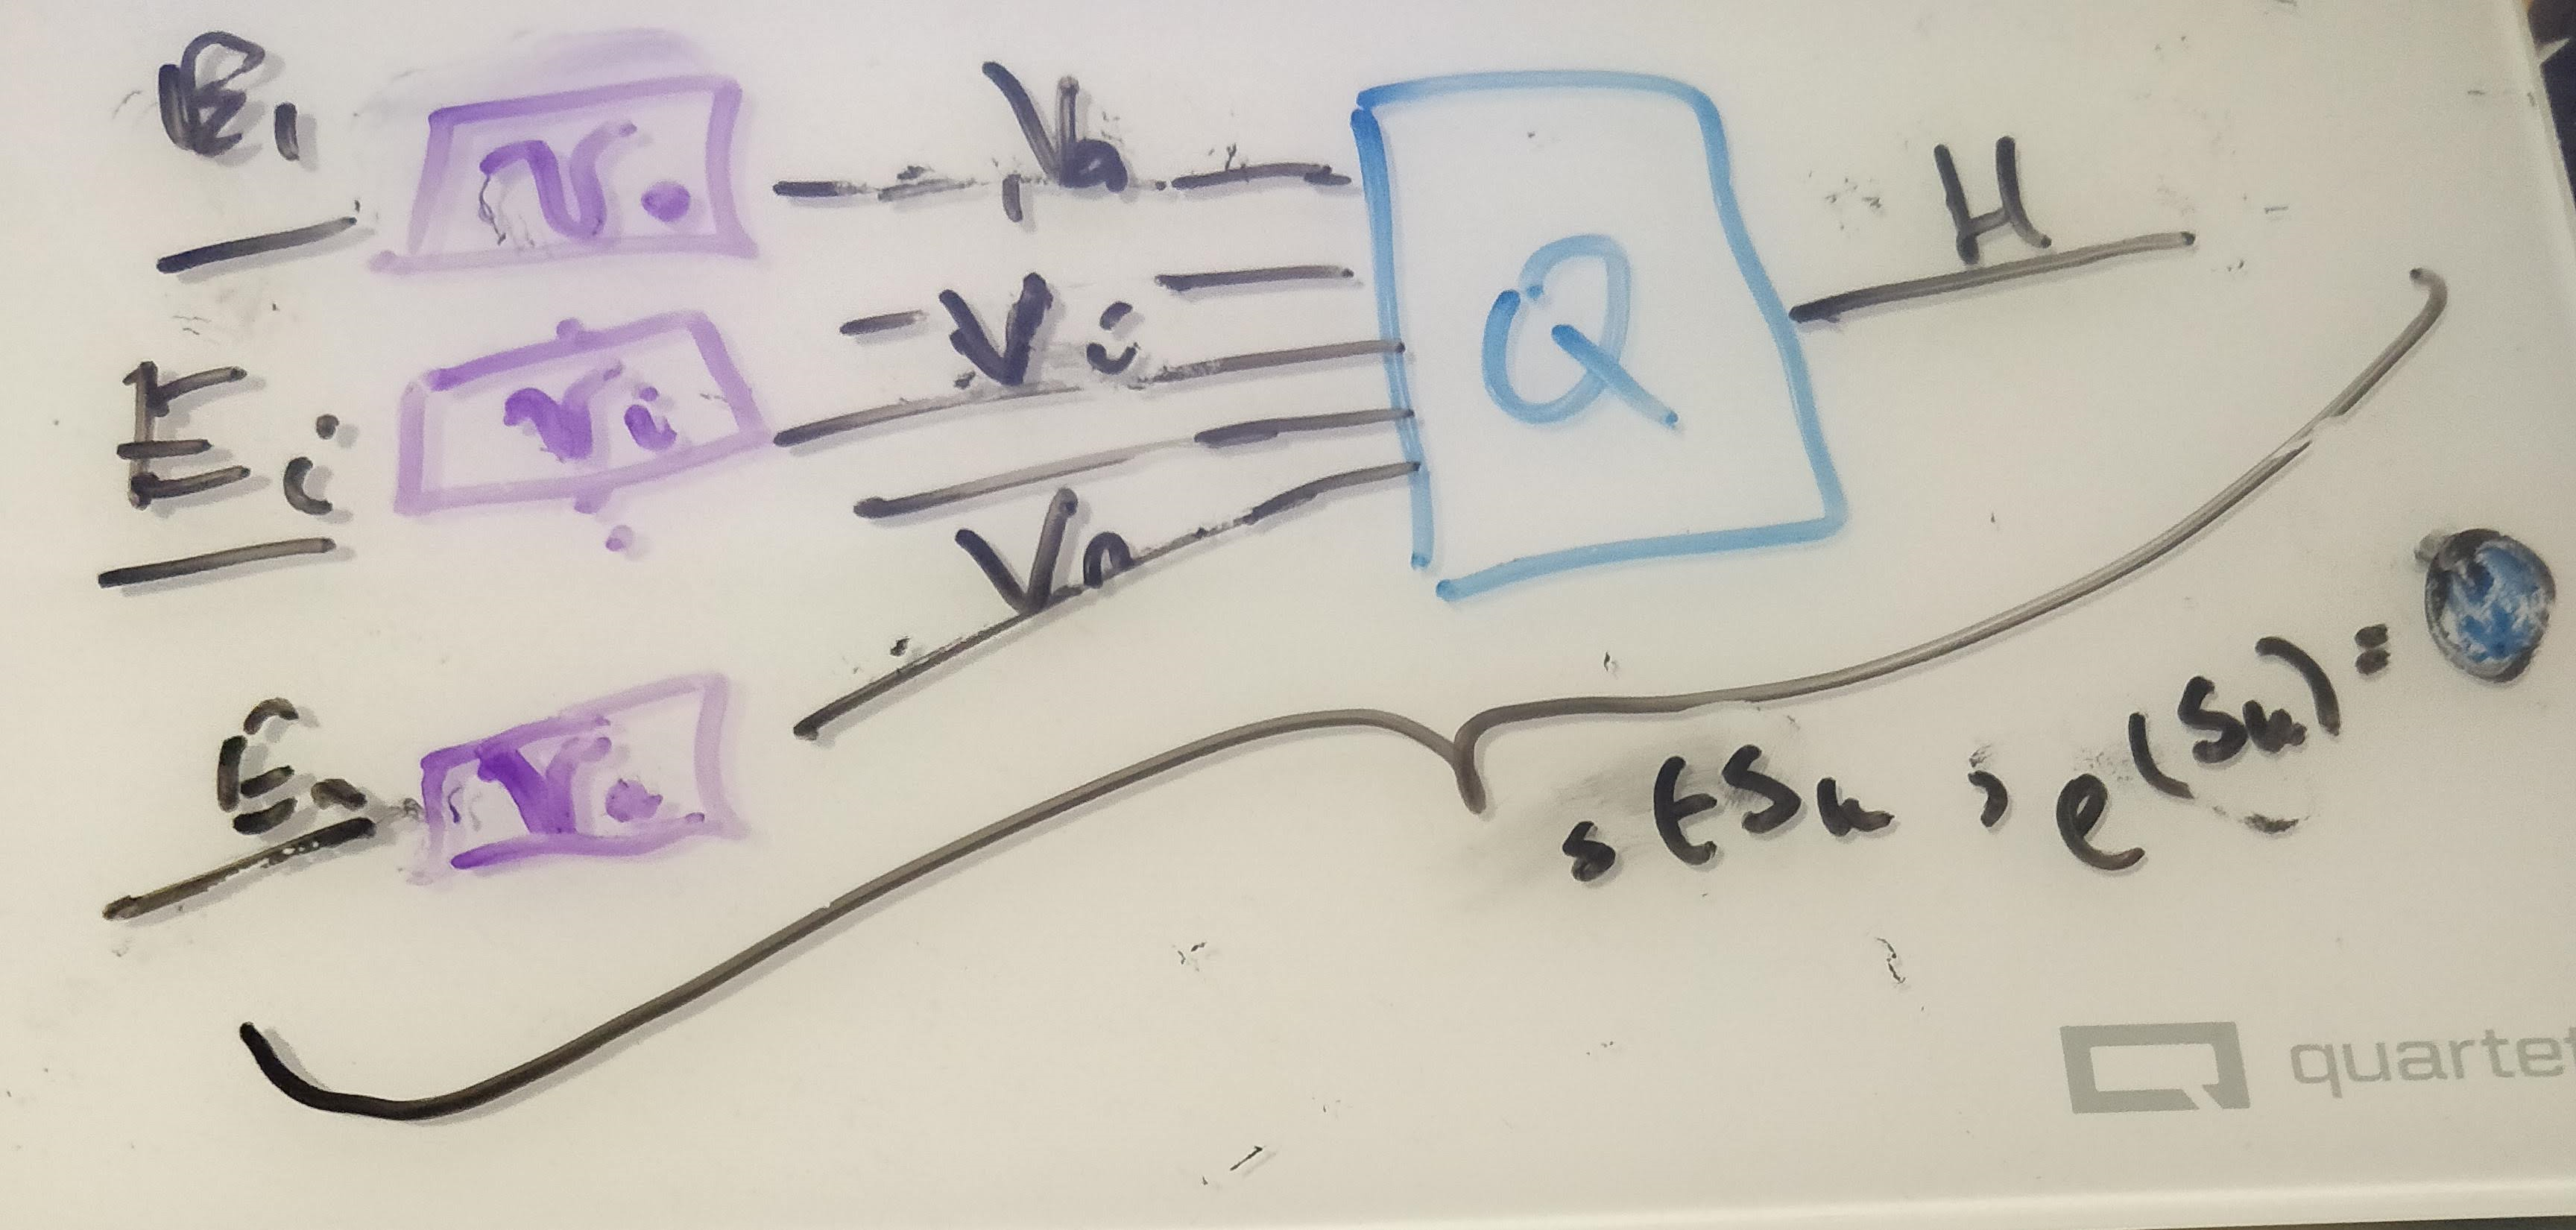
\includegraphics[width=\textwidth]{figures/math/path_of_q}
    \caption{$\vchannel_i$ functions convert data $\dsection_i$ to visual characteristics $\vsection_i$, then \vmark\ assembles $\vsection_i$ into a graphic $\gsection$ such that there is a map \vindex\ preserving the continuity of the data. \gsection\ applied to a region of connected components $\gbase_{\dbasepathpoint}$  generates a part of a graphic, for example the point graphical mark.} 
    \label{fig:artist_q}
\end{figure}

As shown in figure~\ref{fig:artist_q}, the assembly function \vmark\ combines the fiber $\dfiber_i$ wise \vchannel\ transforms into a graphic in \gtotal. Together, \vchannel\ and \vmark\ are a map-reduce operation: map the data into their visual encodings, reduce the encodings into a graphic. As with \vchannel\, the constraint on \vmark\ is that for every monoid action on the input \vsection\, there is corresponding monoid action on the output \gsection. 

While \gsection\ generates the entire graphic, we will restrict the discussion of \vmark\ to generation of sections of a glyph. We formally describe a glyph as \vmark\ applied to the regions \dbasepoint\ that map back to a set of connected components $\dbasepath \subset \dbase$ as input:
\begin{equation}
\dbasepath = \{\dbasepathpoint \in \dbase \text{ s. t. } \exists \gamma \text{ s.t. } \gamma(0)=\dbasepoint \text{ and }\gamma(1)=\dbasepathpoint\}
\end{equation}
where the path\cite{ConnectedSpace2020}  $\gamma$ from \dbasepoint\ to \dbasepathpoint\ is a continuous function from the interval [0,1]. We define the glyph as the graphic generated by $\vmark(\gbase_{\dbasepathpoint})$
\begin{equation}
    \begin{tikzcd}
        \gtotal \arrow[r, shift left] & \gbase_\dbasepathpoint \arrow[rr, "\vindex(\gbasepoint)", shift left] \arrow[l, "\gsection(\gbase_\dbasepathpoint)"] &  & \dbasepath_{\dbasepoint} \arrow[ll, "\vindex^{-1}(\dbasepath)"]
        \end{tikzcd}
    \label{eq:mark}
\end{equation}
such that for every glyph there is at least one corresponding section on \dbase. This is in keeping with the definition of glyph as any differentiable element put forth by Ziemkiewicz and Kosara\cite{ziemkiewiczEmbeddingInformationVisualization2009}. The primitive point, line, and area marks\cite{bertinSemiologyGraphicsDiagrams2011a,carpendaleVisualRepresentationSemiology} are specially cased glyphs.


It is on sections of these glyphs that we define the equivariant map as  $\vmark: \vsection \mapsto \gsection$ and an action on the subset of graphics $\vmark(\Gamma(\vtotal)) \in \Gamma(\gtotal)$ that \vmark\ can generate. We then define the constraint on \vmark such that if \vmark\ is applied to $\vsection, \vsection^{\prime}$ that generate the same \gsection\, then the output of both sections acted on by the same monoid $m$ must be the same. While it may seem intuitive that visualizations that generate the same glyph should consistently generate the same glyph given the same input, we formalize this constraint such that it can be specified as part of the implementation of \vmark. 

Lets call the visual representations of the components $\Gamma(\vtotal)=X$ and the graphic $\vmark(\Gamma(\vtotal))=Y$. If for all monoid actions $m \in \monoid$ and for all $\vsection, \vsection^{\prime} \in X$, the output is equivalent 
\begin{equation}
\vmark(\vsection) = \vmark(\vsection^{\prime})\implies \vmark(m\circ\vsection) = \vmark(m\circ\vsection^{\prime})
\end{equation}
then a monoid action on $Y$ can be defined as $m\circ \gsection = \gsection^{\prime}$. The transformed graphic $\gsection^{\prime}$ is equivariant to a transform on the visual bundle $\gsection^{\prime}=\vmark(m\circ \vsection)$ on a section that $\vsection \in \vmark^{-1}(\gsection)$ that must be part of generating \gsection. 

\begin{figure}[H]
    \includegraphics[width=\textwidth]{figures/math/diff_type_q.png}
    \caption{These two glyphs are generated by the same \vmark\ function. The monoid 
    action $m_i$ on edge thickness $\vsection_i$ of the first glyph yields the thicker edge ${\vsection_i}^{\prime}$ in the second glyph.}
    \label{fig:artist_mark_change}
\end{figure}

The glyph in figure~\ref{fig:artist_mark_change} has the following characteristics \vfiber\ specified by  $(xpos,\, ypos,\, color,\, thickness)$ such that one section is $\vsection=(0,0,0,1)$ and $\vmark(\vsection) = \gsection$ generates a piece of the thin hollow circle. The equivariance constraint on \vmark\ is that the action $m=(e, e, e, x+2)$, where e is identity, translates \vsection\ to  $\vsection^{\prime}=(e,e,e,3)$. The corresponding action on \gsection\ causes $\vmark(\vsection^{\prime})$ to be the thicker circle in figure~\ref{fig:artist_mark_change}.
  

\subsubsection{Assembly \vmark}
In this section we formulate the minimal Q that will generate distinguishable graphical marks: non-overlapping scatter points, a non-infinitely thin line, and an image. 
\begin{figure}[H]
    \includegraphics[width=.75\textwidth]{figures/math/scatter.png}
    \caption{The data is discrete points (temperature, time). Via \vchannel\ these are converted to (xpos, ypos) and pulled over discrete \gbase. These values are then used to parameterize \gsection which returns a color based on the parameters (xpos,ypos) and position $\alpha, \beta$ on $\gbase_{\dbasepoint}$ that \gsection\ is evaluated on. 
    }
    \label{fig:artist_scatter}
\end{figure}
The scatter plot in figure~\ref{fig:scatter} can be defined as $\vmark(xpos, ypos)(\alpha, \beta)$ where color $\gsection_{RGB} = (0,0,0)$ is defined as part of \vmark\ and $\gbasepoint=(\alpha, \beta)$ defines the region on \gbase. The position of this swatch of color can be computed relative to the location on the disc $\gbase_{\dbasepoint}$ as shown in figure~\ref{fig:artist_scatter}:
\begin{align}
x &= size\bullet \alpha \bullet \cos(\beta) + xpos\\
y &= size\bullet \alpha \bullet \sin(\beta) + ypos
\end{align}

such that $\gsection(\gbasepoint) = (x, y, 0, 0, 0)$ colors the point (x,y) black.
\begin{figure}[H]
    \includegraphics[width=.75\textwidth]{figures/math/line.png}
    \caption{The line fiber $(time,\, temp)$ is thickend with the derivative $(time^{\prime},\, temperature^{\prime}$ because that information will be necessary to figure out the tangent to the point to draw a thick line. This is because the line needs to be pushed perpendicular to the tangent of (xpos, ypos). \note{this is gonna move once this gets regenerated w/ labels} The data is converted to visual characteristics (xpos, ypos). The $\alpha$ coordinates on \gbase\ specifies the position of the line, the $\beta$ coordinate specifies thickness.}
    \label{fig:artist_line}
\end{figure}

The line plot $\vmark(xpos, \hat{n_{1}}, ypos, \hat{n_{2}})(\alpha, \beta)$ shown in fig~\ref{fig:artist_scatter} exemplifies the need for the jet. The line needs to know the tangent of the data to draw an envelope above and below each (xpos,ypos) such that the line appears to have a thickness. The magnitude of the thickness is 
\begin{equation}
    \lvert n \rvert = \sqrt{{n_{1}}^2 + {n_{2}}^2}
\end{equation}
such that the normal is  
\begin{equation}
    \hat{n_{1}} = \frac{n_1}{\lvert n \rvert}, \; \hat{n_{2}} = \frac{n_2}{\lvert n \rvert}
\end{equation}

which yields components of \gsection
\begin{align}
 x = xpos(\vindex(\alpha)) &+ \beta\hat{n_1}(\vindex(\alpha)) \\
 y = ypos(\vindex(\alpha)) &+ \beta\hat{n_2}(\vindex(\alpha)) 
\end{align}

where (x,y) look up the position $\vindex(\alpha)$ on the data. At that point, we also look up the the derivatives $\hat{n_1}, \hat{n_2}$  which are then multiplied by data to specify the thickness. 

\begin{figure}[H]
    \includegraphics[width=.75\textwidth]{figures/math/heatmap.png}
    \caption{The only visual parameter a image requires is color since \vindex\ encodes the mapping between position in data and position in graphic. }
    \label{fig:artist_heatmap}
\end{figure}

The image $\vmark(color)$ in figure~\ref{fig:artist_heatmap} is a direct lookup $\vindex:\gbase\rightarrow\dbase$ such that 

\begin{align}
R &= R(\vindex(\alpha, \beta))\\
G &= G(\vindex(\alpha, \beta))\\
B &= B(\vindex(\alpha, \beta))
\end{align}
where \vindex\ may do some translating to a convention expected by \vmark\, for example reorientng the array such that the first row in the data is at the bottom of the graphic. 

\subsubsection{Assembly factory \vmarkd}
The graphic base space \gbase\ is not accessible in many architectures, including Matplotlib; instead we can construct a factory function \vmarkd\ over \dbase\ that can build a \vmark. As shown in eq~\ref{eq:artist_diagram}, \vmark\ is a bundle map $\vmark: \vtotalpull\rightarrow \gtotal$ where \vtotalpull\ and \gtotal\ are both bundles over \gbase.
\begin{figure}[H]
    \includegraphics[width=1\textwidth]{figures/math/q_hat.png}
    \caption{The pullback of the visual bundle \vtotalpull\ is the replication of a \vsection\ over all points \gbasepoint\ that map back to a single \dbasepoint. Because the \vsection\ is the same, we can constract a \vmarkd\ on \vsection\ over \dbasepoint\ that will fabricate the \vmark\ for the equivalent set of \gbasepoint\ associated to that \dbasepoint}
    \label{fig:artist_q_hat}
\end{figure}
 
The preimage of the continuity map $\vpreimg \subset \gbase$ is such that many graphic continuity points $\gbasepoint \in \gbase_{\dbase}$ go to one data continuity point \dbasepoint; therefore, by definition the pull back of \vsection\
\begin{equation}
    \vtotalpull \mid_{\vpreimg} = \vpreimg \times \vfiber
\end{equation}
copies the visual fiber \vfiber\ over the the points \gbasepoint\ in graphic space \gbase\ that correspond to one \dbasepoint\ in data space \dbase\. This set of points \gbasepoint\ are the preimage \vpreimg\ of \dbasepoint. 

This copying is illustrated in figure~\ref{fig:artist_q_hat}, where the 1D fiber $\vfiber \hookrightarrow \vtotal$ over \dbase\ is copied repeatedly to become the 2D fiber $\vfiberpull \hookrightarrow \vtotalpull$ with identical components over \gbase. Given the section \vsectionpull\ pulled back from \vsection\ and the point $\gbasepoint \in \vpreimg$, there is a direct map from \vsection on a point \dbasepoint, there is a direct map from the visual section over data base space  $(\dbasepoint, \vsection(\dbasepoint)) \mapsto (\gbasepoint, \vsectionpull(\gbasepoint))$ to the visual section \vsectionpull\ over graphic base space. This map means that the pulled back section $\vsectionpull(\gbasepoint) = \vindex^*(\vsection(\dbasepoint))$ is the section \vsection\ copied over all \gbasepoint. This means that \vsectionpull\ is identical for all \gbasepoint\ where $\vindex(\gbasepoint) = \dbasepoint$, which is illustrated in figure~\ref{fig:artist_q_hat} as each dot on \vfiber is equivalent to the line intersection \vfiberpull. 

Given the equivalence between \vsection\ and \vsectionpull\ defined above, the reliance on \gbase\ can be factored out. When \vmark\ maps visual sections  into graphics $\vmark: \Gamma(\vtotalpull) \rightarrow \Gamma(\gtotal)$, if we restrict \vmark\ input to the pulled back visual section \vsectionpull\ then 
\begin{equation}
    \gsection(\gbasepoint) \coloneqq \vmark(\vsectionpull)(s)
\end{equation}
the graphic section \gsection\ evaluated on a visual region \gbasepoint\ is defined as the assembly function \vmark\ with input pulled back visual section \vsectionpull\ also evaluated on \gbasepoint. Since the pulled back visual section \vsectionpull\ is the visual section \vsection\ copied over every graphic region $\gbasepoint \in \vpreimg$, we can define a \vmark\ factory function 
\begin{equation}
\vmarkd(\vsection(\dbasepoint))(\gbasepoint) \coloneqq \vmark((\vsectionpull)(\gbasepoint))
\end{equation} 
where the assembly function \vmarkd\ that takes as input the visual section on data \vsection\ is defined to be the assembly function \vmark\ that takes as input the copied section \vsectionpull\ such that both functions are evaluated over the same location $\vpreimg = \gbasepoint$ in the base space \gbase. 

Factoring out \gbasepoint\, $\vmarkd(\vsection(k)) = \vmark(\vsectionpull)$ generates a curried \vmark. In fact, \vmarkd\ is a map from visual space to graphic space $\vmarkd:\Gamma(\vtotal) \rightarrow \Gamma(\gtotal)$ locally over \dbasepoint\ such that it can be evaluated on a single visual record   $\vmarkd:\Gamma(\vtotal_{\dbasepoint}) \rightarrow \Gamma(\gtotal\mid_{\vpreimg})$. This allows us to construct a \vmarkd\ that only depends on \dbase, such that for each $\vsection(\dbasepoint)$ there is part of $\gsection\mid_{\vpreimg}$. The construction of \vmarkd\ allows us to retain the functional map reduce benefits of \vmark\ without having to majorly restructure the existing rendering pipeline.

\subsubsection{Sheaf}
\label{sec:artist_sheaf_stalk}
The restriction maps of a sheaf describe how local \dsection can be glued into larger sections \cite{ghristElementaryAppliedTopology2014,ghristHomologicalAlgebraData2018}. As part of the definition of local triviality, there is an open neighborhood $U\subset \dbase$ for every $\dbasepoint \in \dbase$. We can define the inclusion map $\iota: U \rightarrow \dbase$  which pulls \dtotal over $U$ 
\begin{equation}
    \label{eq:sheaf}
    \begin{tikzcd}
        \iota^*\dtotal \arrow[d, "\pi"'] \arrow[r, "\iota^*", hook]             & \dtotal \arrow[d, "\pi"']                  \\
        U \arrow[r, "\iota", hook] \arrow[u, "\iota^{*}\dsection"', bend right] & \dbase \arrow[u, "\dsection"', bend right]
    \end{tikzcd}
\end{equation}
such that the pulled back $\iota^*\dsection$ only contains records over $U \subset \dbase$. By gluing $\iota^*\dsection$ together, the sheaf is putting a continuous structure on local sections which allows for defining a section over a subset in \dbase. That section over subset \dbase\ maps to the graphic generated by \vartist\ for visualizations such as sliding windows\cite{crouchDynamicGraphsSlidingwindow2013,chuTimeSeriesSegmentation1995} streaming data, or navigation techniques such as pan and zoom\cite{NekrasovskiEvaluationPanZoom2006}.


\subsubsection{Composition of Artists: +}
\begin{figure}
    \includegraphics[width=1\textwidth]{figures/math/addition_operator.png}
    \caption{$\dsection_1$ and $\dsection_2$ are distinct datasets passed through artists $\vartist_1$ and $\vartist_2$ to generate graphics $\gsection_1$ and $\gsection_2$. These graphics happen to be rendered to the same image, but otherwise have no intrinsinc link.}
    \label{fig:artist_plus}
\end{figure}
To build graphics that are the composites of multiple artists, we define a simple addition operator that is the disjoint union of fiber bundles \dtotal.  For example, in figure~\ref{fig:artist_plus} the scatter plot $\dtotal_1$ and the line plot $\dtotal_2$ have different \dbase that are mapped to separate \gbase. To fully display both graphics, the composite graphic $\vartist_1 + \vartist_2$ needs to include all records on both $\dbase_1$ and $\dbase_2$, which are the sections on the disjoint union $\dbase_1 \sqcup \dbase_2$. This in turn yields disjoint graphics $\gbase_1 \sqcup \gbase_2$ rendered to the same image. Constraints can be placed on the disjoint union such as that the fiber components need to have the same \vchannel position encodings or that the position \vsection need to be in a specified range. There is a second type of composition where $\dtotal_1$ and $\dtotal_2$ share a base space $\dbase_2 \hookrightarrow \dbase_1$ such that the the artists can be considered to be acting on different components of the same section. This type of composition is important for creating visualizations where elements need to update together in a consistent way, such as multiple views \cite{alboRadarComparativeEvaluation2016a, hullmanKeeping2018} and brush-linked views\cite{beckerBrushingScatterplots1987,bujaInteractiveData1991}. 

\subsubsection{Equivalance class of artists $\vartist^{\prime}$}
\label{sec:artist_equivalance}
It is impractical to implement an artist for every single graphic; instead we implement an approximation of an the equivalence class of artists $\{\vartist \in \vartist^{\prime}: \vartist_{1} \equiv \vartist_{2}\}$. Roughly, equivalent artists have the same fiber bundle \vtotal\ and same assembly function \vmark\ but act on different sections \vsection, but we will formalize the definition of the equivalance class in future work. 

As a first pass for implementation purposes, we identify a minimal \vfiber\ associated with each $\vartist^{\prime}$ that defines what visual characteristics of the graphic must originate in the data such that the graphic is identifiable as a given chart type.
%%
%%\begin{figure}[H]
%%   \caption{Each of these graphics is generated by a different artist \vartist which is the equivalance class of scatter plots $\vartist^{\prime}$\note{this is gonna be a whole bunch of scatter plots}}
%%    \label{fig:artist_equivalence}
%%\end{figure}

For example, a scatter plot of red circles is the output of one artist, a scatter plot of green squares the output of another. These two artists are equivalent since their only difference is in the literal visual encodings (color, shape). Shape and color could also be defined in \vmark\, but the position must come from the fiber $\vfiber=(xpos,ypos)$ since fundementally a scatter plot is the plotting of one position against another\cite{friendlyBriefHistoryData2008}. We also use this criteria to identify derivative types, for example the bubble chart\cite{tufteVisualDisplayQuantitative2001} is a type of scatter where by definition the glyph size is mapped from the data. The criteria for equivalence class membership serves as the basis for evaluating invariance\cite{kindlmann2014algebraic}. 
\end{document}